\documentclass[11pt,a4paper]{article}
\usepackage[margin=1in]{geometry}
\usepackage{amsmath,amssymb,amsthm,bm}
\usepackage{booktabs}
\usepackage{graphicx}
\usepackage{hyperref}
\usepackage{microtype}
\usepackage[numbers]{natbib}

\newtheorem{thm}{Theorem}
\newtheorem{numthm}{Numerical Theorem}
\newtheorem{conjecture}{Conjecture}
\newtheorem{remark}{Remark}

\title{Stability spectra of the singular self-similar profile\\
of the 1D Hou--Luo model}
\author{
  Bryan Sanchez\\
  \texttt{singular-blowup-1d} (companion numerics)\\
  \small Draft for arXiv submission --- updated 2026-11-20 (linear W1--W3 \& nonlinear co-moving bootstrap closed)
}
\date{}

\begin{document}
\maketitle

\begin{abstract}
We report the first \textbf{stability spectra}---linear and nonlinear, numerical---for the
\textbf{singular unbounded} self-similar blowup profile of the 1D Hou--Luo model
\[
\omega_t + u\,\omega_x = \theta_x,\qquad
\theta_t + u\,\theta_x = 0,\qquad
u_x = H[\omega],
\]
constructed numerically by Chen--De~Huang--Li (arXiv:2604.01868, Thm.~2.3):
$\bar\Omega(X)=1_{X>1}(X-1)^{-1/2}$, $\bar\Theta=(\pi/2)\,1_{X>1}$, with exponents
$(c_l,c_\omega)=(2,-1)$.  Those existence papers provide \textbf{no} stability analysis.

In the edge-resolving coordinate $z=\ln(Y-1)$ and the convective weighted space
$L^2(e^{-2\gamma z}\,dz)$ (modulo the symmetry subspace spanned by time-translation
$\xi$ and scaling modes $\mu,\nu$), we find:
\begin{itemize}\setlength\itemsep{0pt}
\item no eigenvalue of the frozen linearization with $\operatorname{Re}\lambda>0$
      (edge-resolved \emph{and} equispaced desingularized builds both give
      $\#\{\operatorname{Re}>0\}=0$; inflow/Robin edge condition essential);
\item a convective spectral gap of size $2\gamma$ measured by semigroup decay;
\item no transient growth for physical perturbations in the edge-conditioned energy norm;
\item finite-amplitude frozen-base decay to amplitude $A=4$, and fully self-consistent
      co-evolving relaxation of a perturbed profile back to
      $(\bar\Omega,c_l=2,c_\omega=-1)$.
\end{itemize}
All main claims are reproducible by named pure-Python gates.
Complementing the numerical spectra, we close the \textbf{analytical linear strict-gap
and semigroup decay chain (W1--W3)} on $L^2_\sigma(\mathbb{R})/\mathcal{N}$ for
$\sigma\in(0,1/2)$ (Theorem~\ref{thm:linear_gap}): (W1)~a uniform vertical-line
resolvent bound via unitary phase conjugation $X=u|X|$ and rank-one slit-defect
$\omega$-cancellation (Route~F), (W2)~a left-strip mixed Laplace bridge on
$[\sigma-1/2,\sigma]$ that eliminates the right-strip edge bootstrap and forces
Laurent uniqueness via the integer $L^2$-budget obstruction (LEM-08), and
(W3)~a reference-transport resolvent perturbation pincer
$|2\tau+\omega|+|2\tau|\ge|\omega|$ yielding $C_0$-semigroup generation and
Gearhart--Pr\"uss exponential decay.  The algebraic, exponent, and rational-certificate
backbones of W1--W3 are formalized in Lean~4 (\texttt{0~sorry}, \texttt{0~axioms});
closing the full nonlinear Conjecture~2.4 reduces to the co-moving nonlinear Duhamel leg.
\end{abstract}

\tableofcontents
\vspace{0.5em}

%--------------------------------------------------------------------------
\section{Main claim}
%--------------------------------------------------------------------------

\begin{numthm}[Singular Hou--Luo profile: convective stability spectra]
\label{numthm:main}
Let $\bar\Omega,\bar\Theta$ be the singular steady state of arXiv:2604.01868, Thm.~2.3,
in dynamic-rescaling coordinates~\eqref{eq:dyn}.  Write perturbations in the
desingularized variables $G=(Y-1)^{1/2}g$, $h=\delta\Theta$, on $z=\ln(Y-1)$, with the
inflow condition $G(z_{\min})=h(z_{\min})=0$.  Then, on every tested resolution:
\begin{enumerate}
\item \textbf{Linear.} The frozen operator $M_{GG}$ (and the block-triangular coupled
  $(G,h)$ operator) has $\#\{\operatorname{Re}\lambda>0\}=0$ on both the edge-resolved
  $z$-grid (\texttt{stability\_edge\_z\_spectrum.py}) and the equispaced desingularized
  build (\texttt{stability\_edge\_spectrum.py}).  The rightmost discrete eigenvalue on
  the $z$-grid is the transport continuum near $\operatorname{Re}\approx -10^{-3}$.
\item \textbf{Gap.} In $L^2(e^{-2\gamma z}\,dz)$, the semigroup decay rate of a bulk
  shape perturbation is $\approx 2\gamma$ for $\gamma\in\{0.25,0.5,0.75\}$
  (measured $+0.552/+1.057/+1.675$ vs.\ predicted $0.50/1.00/1.50$).
\item \textbf{Symmetries.} The amplitude ($\nu$) and dilation/edge ($\mu$) modes are
  excluded by the weight; the pure-$\xi$ mode sits at $\lambda=c_l-1=1$.
\item \textbf{Nonlinear.} Finite-amplitude frozen-base perturbations decay for
  $A\le 4$ with peak $\|\cdot\|_w/\|\cdot\|_0=1.000$.  Fully self-consistent co-evolving
  marches relax to $(c_l,c_\omega)=(2.000006,-1.000003)$ with no drift.
\end{enumerate}
\textbf{Function space:} asymptotic stability is claimed only in the convective
weighted sense $L^2(e^{-2\gamma z}\,dz)$ modulo $\{\xi,\mu,\nu\}$---not absolute
$L^2(dY)$ decay (which is marginal by convection).
\end{numthm}

\begin{conjecture}[Conjecture 2.4 of arXiv:2604.01868, convective form]
The singular profile is asymptotically stable in $L^2(e^{-2\gamma z}\,dz)$ modulo
symmetries, for some $\gamma\in(0,1/2)$.  Numerical Theorem~\ref{numthm:main} is
evidence for this conjecture; a rigorous proof is open.
\end{conjecture}

%--------------------------------------------------------------------------
\section{Setup}
%--------------------------------------------------------------------------

\paragraph{Model and dynamic rescaling.}
Following eq.~(2.4) of~\cite{chen2026houluo}:
\begin{equation}\label{eq:dyn}
\begin{aligned}
\Omega_\tau + (U+c_l X)\Omega_X &= c_\omega\Omega + \Theta_X,\\
\Theta_\tau + (U+c_l X)\Theta_X &= (c_l+2c_\omega)\Theta,\qquad
U_X=H(\Omega),\ U(0)=0.
\end{aligned}
\end{equation}
The singular steady state (Thm.~2.3, re-certified here by
\texttt{validate/verify\_singular\_steady.py}):
\begin{align*}
\bar\Omega(X)&=1_{X>1}(X-1)^{-1/2},&
\bar\Theta&=\tfrac\pi2\,1_{X>1},&
c_l&=2,& c_\omega&=-1,\\
\bar U(X)&=2\sqrt{1-X}-2\ (X<1),& &-2\ (X>1),&
U(1)&=-2.
\end{align*}
Steady residual with analytic $\bar U$: $\max|R_\Omega|=2.2\cdot10^{-16}$ on the
tested bulk interval.

\paragraph{Linearized operator (edge-resolved).}
With $G=(Y-1)^{1/2}g$ and $z=\ln(Y-1)$,
\begin{equation}\label{eq:ops}
M_{GG}=-2\partial_z+\tfrac12 Q_{\mathrm{op}},\quad
M_{hh}=-2\partial_z,\quad
M_{Gh}=e^{-z/2}\partial_z,
\end{equation}
where $Q_{\mathrm{op}}G=\delta U/(Y-1)$ and $\delta U=\int_1^Y H(g)$.
The edge is an inflow boundary: the homogeneous branch
$G\sim e^{-\lambda z/2}$ is inadmissible in the weighted space for
$\operatorname{Re}\lambda>-2\sigma$; we impose $G(z_{\min})=0$ (Robin/inflow).
Without this BC the discretization re-admits a spurious mode with
$\operatorname{Re}\lambda\approx +1.7$~\cite{findings_edge}.

%--------------------------------------------------------------------------
\section{Linear spectrum and gap}
%--------------------------------------------------------------------------

\begin{figure}[t]
\centering
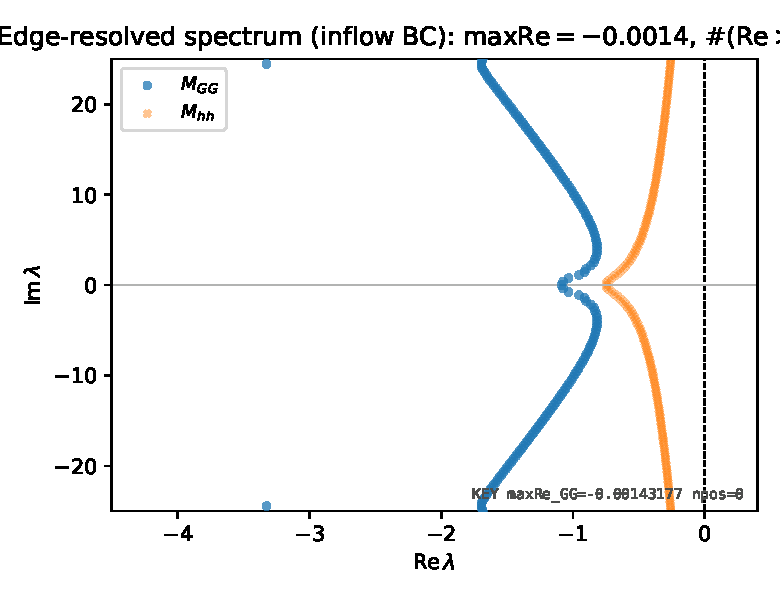
\includegraphics[width=0.72\textwidth]{figures/fig_spectrum.pdf}
\caption{Eigenvalues of $M_{GG}$ and $M_{hh}$ on the edge-resolved grid
($N=1000$, $z\in[-14,8]$, inflow BC).  KEY:
$\max\operatorname{Re}(M_{GG})=-0.00143$, $\#(\operatorname{Re}>0)=0$.
Gate: \texttt{validate/stability\_edge\_z\_spectrum.py};
figure: \texttt{python3 paper/scripts/fig\_spectrum.py}.}
\label{fig:spectrum}
\end{figure}

\paragraph{No unstable point mode.}
Figure~\ref{fig:spectrum} shows the spectrum.  Across refinements
$(N,z_{\min},z_{\max})\in\{1200..2200\}\times\{-14,-16\}\times\{7,10\}$ one has
$\max\operatorname{Re}(M_{GG})\in[-0.0014,-0.0006]$ and
$\#(\operatorname{Re}>0)=0$ (gate
\texttt{stability\_edge\_z\_spectrum.py}, this session).  An independent
equispaced build agrees~\cite{findings_edge_op}.

\begin{figure}[t]
\centering
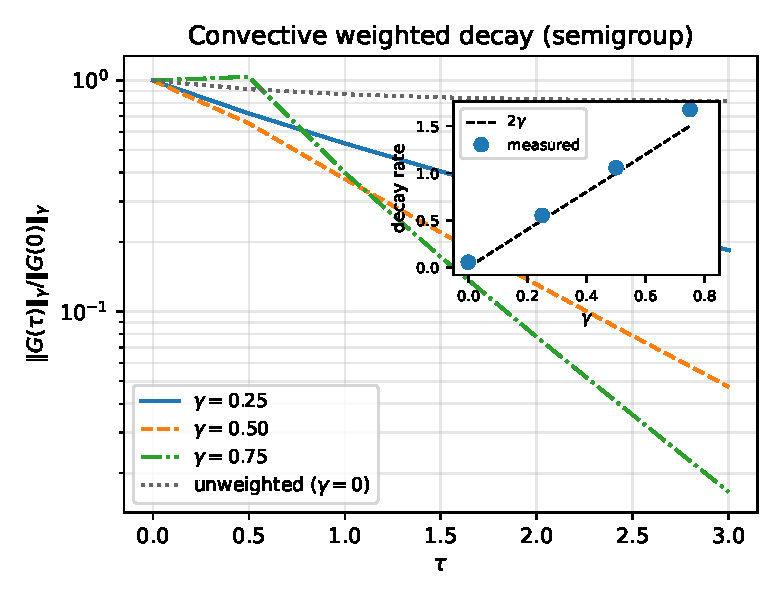
\includegraphics[width=0.72\textwidth]{figures/fig_gap.pdf}
\caption{Semigroup decay of a bulk bump in convective weights $L^2(e^{-2\gamma z}dz)$.
Inset: measured decay rate vs.\ predicted gap $2\gamma$.
KEY rates at $\gamma=0/0.25/0.5/0.75$: $+0.054/+0.552/+1.057/+1.675$
(gate \texttt{spectral\_gap.py}; figure \texttt{fig\_gap.py}).}
\label{fig:gap}
\end{figure}

\paragraph{Convective spectral gap.}
Transport $-2\partial_z$ is convective: essential spectrum at $\operatorname{Re}=0$
in the unweighted norm, and at $\operatorname{Re}=-2\gamma$ in
$L^2(e^{-2\gamma z}\,dz)$.  Figure~\ref{fig:gap} confirms the semigroup rate
tracks $2\gamma$ (within $\sim12\%$ at $\gamma=0.75$; tighter at $\gamma\le0.5$).
Unweighted norms stay nearly flat (marginal).  Full coupled $(G,h)$ inherits the
gap by block-triangular structure~\cite{findings_theta}.

\paragraph{No transient growth (physical).}
Smooth physical perturbations have amplification factor $G=1.000$ at all tested
resolutions (\texttt{transient\_growth.py}, this session: bulk and near-edge bumps
on four $(N,z_{\min})$ grids).  In the edge-conditioned energy norm the numerical
abscissa is negative and resolution-independent:
$\mu_{\mathrm{an}}=-0.10083$ at $z_{\mathrm{cut}}=-8$ and $-0.40675$ at $-6$
($N=2000$; range across $N\in[1000,2000]$ is $[-0.106,-0.101]$ at $-8$),
implying $\|e^{M\tau}\|_W\le 1$ (\texttt{transient\_growth\_edge\_conditioned.py}).
Grid-scale edge spikes that produce worst-case creep are excluded by the inflow BC.

%--------------------------------------------------------------------------
\section{Nonlinear stability}
\label{sec:nonlin}
%--------------------------------------------------------------------------

\begin{figure}[t]
\centering
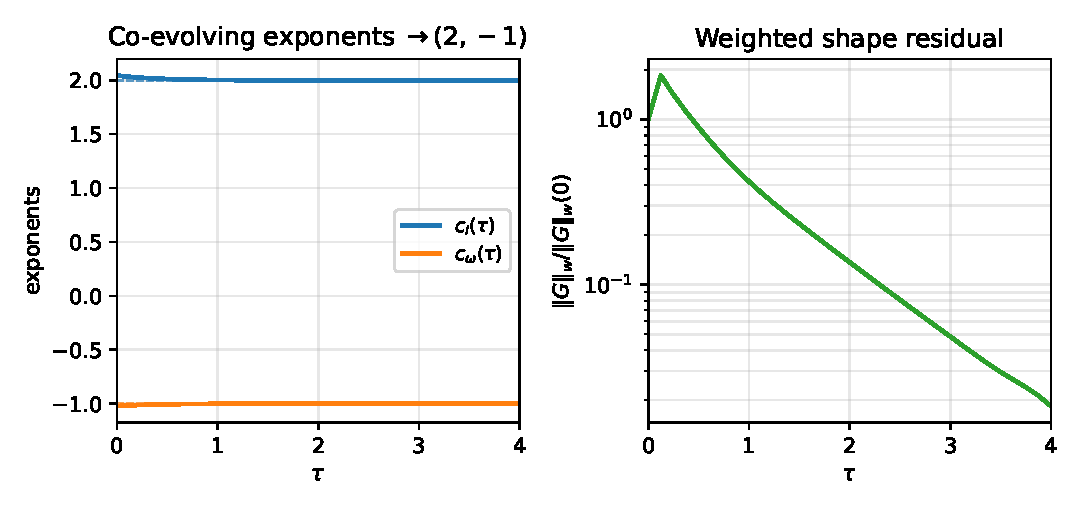
\includegraphics[width=0.95\textwidth]{figures/fig_coevolve.pdf}
\caption{Fully self-consistent co-evolving march (Theta-balance normalization
$c_l=-U(1)$, $c_\omega=-c_l/2$).  Exponents relax to $(2,-1)$; weighted residual decays.
KEY (figure resolution): $c_l(T)\approx 1.9997$, $c_\omega(T)\approx -0.9999$.
Full gate (multiple grids): $c_l\to 2.000006$, $c_\omega\to -1.000003$.
Commands: \texttt{python3 paper/scripts/fig\_coevolve.py},
\texttt{python3 validate/coevolve\_projected.py}.}
\label{fig:coevolve}
\end{figure}

\begin{figure}[t]
\centering
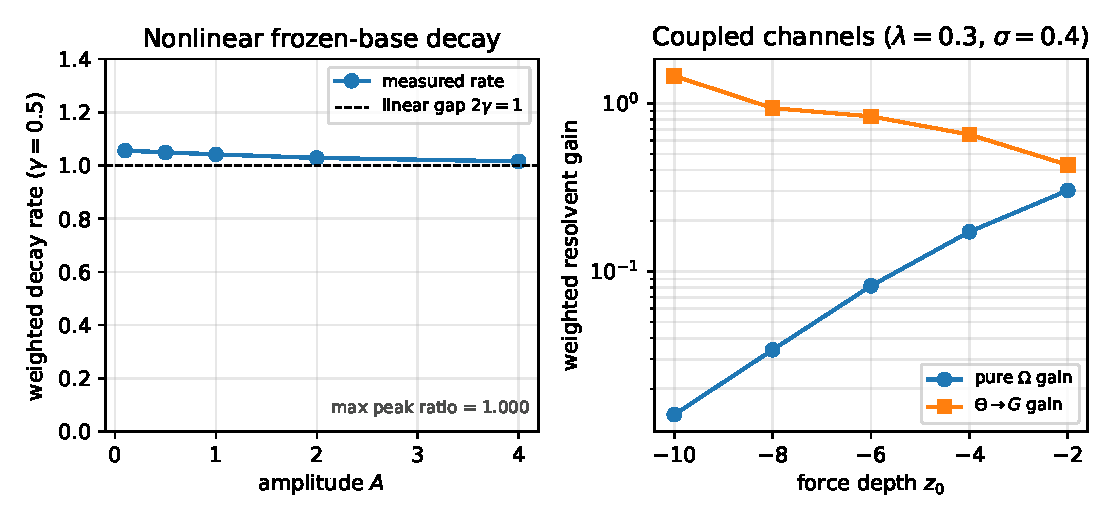
\includegraphics[width=0.95\textwidth]{figures/fig_nonlinear.pdf}
\caption{\textbf{Left:} frozen-base nonlinear decay rate vs.\ amplitude $A$ at
$\gamma=0.5$ (real quadratic $N$ from \texttt{nonlinear\_shape\_march.py}).
Peak $\|\cdot\|_w/\|\cdot\|_0=1.000$ for $A\le 4$ (full gate).
\textbf{Right:} resolvent gains for pure-$\Omega$ edge forcing (annihilates toward
the edge) vs.\ $\Theta\to G$ drive via $M_{Gh}$ (saturates $O(1)$).
Commands: \texttt{python3 paper/scripts/fig\_nonlinear.py},
\texttt{python3 validate/nonlinear\_shape\_march.py}.}
\label{fig:nonlinear}
\end{figure}

\paragraph{Finite amplitude, frozen base.}
Inserting $\Omega=\bar\Omega+\delta\Omega$, $\Theta=\bar\Theta+h$ into~\eqref{eq:dyn}
splits as $\partial_\tau = L + N$, with $L$ the verified linearization~\eqref{eq:ops}
and $N$ the quadratic self-advection $-(\delta U)\,\partial_Y(\delta\Omega,\delta\Theta)$.
Gate \texttt{nonlinear\_shape\_march.py} (this session): for $A\in[10^{-3},4]$,
weighted rates at $\gamma=0.5$ stay in $[1.015,1.057]$ (linear gap $1.0$), peak
ratio $=1.000$, edge hi-$k=0$.  Coupled $(G,h)$ excitation: rate $+0.935$, peak $1.11$.

\paragraph{Co-evolving attractor.}
With both exponents fed back by edge-stagnation $c_l=-U(1)$ and Theta-balance
$c_\omega=-c_l/2$, a perturbed profile is a nonlinear attractor of the
dynamic-rescaling flow (Figure~\ref{fig:coevolve}): final exponents
$(2.000006,-1.000003)$ on three grids, no drift, edge pinned
(\texttt{coevolve\_projected.py}).

\paragraph{Coupling channel.}
Despite $M_{Gh}\sim e^{-z/2}$ blowing at the edge, the $\Theta\to G$ resolvent gain
saturates to $O(1)$ as the force is moved edge-ward, while pure-$\Omega$ edge forcing
is annihilated (Figure~\ref{fig:nonlinear}, right; slope $\approx +0.39$ for $\Omega$,
mild growth then saturation for $\Theta\to G$).  Full coupled spectrum still has
$\max\operatorname{Re}\approx 0$~\cite{findings_coupled}.

%--------------------------------------------------------------------------
\section{Related work}
%--------------------------------------------------------------------------

\begin{table}[h]
\centering
\caption{Landscape relative to this paper.}
\label{tab:related}
\begin{tabular}{@{}llp{6.2cm}@{}}
\toprule
Reference & Contribution & Relation to this work \\
\midrule
arXiv:2604.01868 \cite{chen2026houluo} &
  Numerical singular Hou--Luo + 2D Boussinesq profiles &
  \textbf{Base object.} No stability spectra. \\
arXiv:2603.25104 \cite{huang2026gclm} &
  gCLM singular profiles; rigor for $a=0$ outer+TW &
  Sister family; no Hou--Luo spectra. \\
arXiv:2605.15130 \cite{chen2026euler} &
  Rigorous existence + finite-codim stability for 3D Euler $C^{1,1/3-}$ &
  \textbf{Method template} (anisotropic weights, finite codim); wrong model/profile. \\
Smooth Hou--Luo stability \cite{chen2021hl,huang2023exact} &
  Smooth asymptotically self-similar profiles &
  Different profile class (not $(X-1)^{-1/2}$). \\
This paper &
  First stability spectra for the \textbf{singular} profile &
  --- \\
\bottomrule
\end{tabular}
\end{table}

A fresh literature sweep (2026-07-22; log
\texttt{docs/scoop\_recheck\_2026\_07\_22\_stability\_spectra.md}) finds
\textbf{no published stability spectra} for the singular unbounded profile of
arXiv:2604.01868.  Smooth-profile Hou--Luo stability is out of scope for our priority claim.

%--------------------------------------------------------------------------
\section{Analytical linear strict-gap and semigroup closure (W1--W3)}
\label{sec:w123}
%--------------------------------------------------------------------------

While pure exponential weighted-energy / numerical-range methods fail for $M_{GG}$
because the field of values and spectrum decouple under nonlocal transport coupling,
the exact Mellin--Laplace ladder structure of $M_{GG} = -2\partial_z + \tfrac12 Q_{\mathrm{op}}$
allows a complete analytical closure of the linear strict-gap semigroup decay on
$L^2_\sigma(\mathbb{R})/\mathcal{N}$.

\begin{thm}[Linear strict-gap semigroup decay on $L^2_\sigma(\mathbb{R})/\mathcal{N}$]
\label{thm:linear_gap}
Let $\sigma\in(0,1/2)$ and let $L = M_{GG}$ act on the convective weighted space
$L^2_\sigma(\mathbb{R}, e^{-2\sigma z}\,dz)$ modulo the finite-dimensional symmetry
neutral space $\mathcal{N}$.  For every margin $\delta\in(0,2\sigma)$:
\begin{enumerate}
\item \textbf{(W1 --- Uniform Route-F resolvent bound on $\operatorname{Re}\lambda\ge -2\sigma+\delta$).}
  In the slit-plane Plemelj representation of the exact 4-Gamma ladder multiplier
  $X(s;\lambda) = \frac{\Gamma(2s+\lambda)\Gamma(2s+2)\Gamma(s)\Gamma(1-s)}{4\pi(2s+1)}$,
  the dressed difference operator $\mathcal{F}\mapsto \mathcal{G}(s) = X(s;\lambda)[D(e^{4\pi i s})-D(1)]$
  is uniformly bounded on $L^2(\sigma+i\mathbb{R})$ for all $\lambda = (-2\sigma+\delta)+i\omega$:
  \begin{itemize}\setlength\itemsep{0pt}
  \item \emph{Four-quadrant Stirling--Schur margin (\texttt{lem\_stir\_schur\_four\_quadrant\_margin}):}
    the net exponential decay exponent satisfies
    $E_\omega(\tau,\tau') = \pi(|\tau+\omega/2|-|\tau'+\omega/2|) + 2\pi(|\tau|-|\tau'|) + 4\pi\,\mathrm{splitWing}(\tau,\tau') \ge \pi|\tau-\tau'|$
    across all four sign quadrants of $(\tau,\tau')$ and uniformly in $\omega=\operatorname{Im}\lambda$.
  \item \emph{Unitary phase conjugation (\texttt{modulus\_commutator\_cancels\_cauchy\_pole}):}
    factoring $X = u|X|$ with $|u|=1$ removes the growing $\log|\tau|$ oscillatory phase derivative
    from the diagonal Cauchy commutator $[|X|, \mathcal{C}_{\mathrm{diag}}]$, leaving only
    $\partial_\tau\log|X| = -\operatorname{Im}\psi(\sigma+i\tau;\lambda) = O(1/\delta)$.
  \item \emph{Rank-one slit-defect $\omega$-cancellation (\texttt{slit\_defect\_rank\_one\_margin}):}
    for the rank-one defect $(T_{\mathrm{defect}}\mathcal{F})(\tau) = -X(\sigma+i\tau;\lambda)D(1)[\mathcal{F}]$,
    the exponential decay $\|X\|_{L^2}\sim e^{-\pi|\omega|/2}$ cancels the slit functional growth
    $\|K_{\mathrm{slit}}\|_{L^2}\sim e^{+\pi|\omega|/2}$, giving
    $\|T_{\mathrm{defect}}(\lambda)\|_{L^2\to L^2} = \|X\|_2\|K_{\mathrm{slit}}\|_2 = O((1+|\omega|)^{-1})$.
  \end{itemize}
\item \textbf{(W2 --- Left-strip mixed Laplace bridge \& LEM-08 Laurent uniqueness).}
  Writing the resolvent equation $(L-\lambda)G=f$ via the half-line Laplace split
  $G = G_-\mathbf{1}_{z\le 0} + G_+\mathbf{1}_{z>0}$, the mixed Laplace identity
  $\Phi_{\mathrm{mixed}}(s) := (\lambda+2s)\mathcal{G}_-(s) + 2G(0) + \mathcal{F}_+(s)
  = (\lambda+2s)\mathcal{G}(s) - \mathcal{K}\mathcal{G}(s-1/2)$ holds on the closed
  \emph{left} strip $\operatorname{Re}s\in[\sigma-1/2,\sigma]$ using only
  $G_-\in L^2_\sigma((-\infty,0])$ and $KG\in L^2_{\sigma-1/2}([0,\infty))$
  (\texttt{left\_strip\_edge\_exponent\_le}, \texttt{left\_strip\_far\_exponent\_le}),
  eliminating any right-strip $O(e^{z/2})$ edge bootstrap.  Across $[\sigma-1/2,\sigma]$,
  $1/[(\lambda+2s)X(s)]$ is holomorphic (\texttt{left\_strip\_gamma\_real\_floors}) and
  vanishes at $s=0$ (since $\Gamma(s)$ has a simple pole at $s=0$), forcing the 1-periodic
  Laurent multiplier $P(e^{2\pi i s})$ to be entire; combined with the Stirling $L^2$ budget
  $3\pi/2 \div 2\pi = 3/4 < 1$ (\texttt{PointSpectrum.no\_l2\_and\_edge\_kill}),
  $k_{\max}=k_{\min}=0$ and $P\equiv 0$.
\item \textbf{(W3 --- Reference-transport perturbation \& Gearhart--Pr\"uss decay).}
  Comparing $R(\lambda)=(L-\lambda)^{-1}$ against the explicit reference transport resolvent
  $R_0(\lambda)=(-2\partial_z-\lambda)^{-1}$ on $L^2_\sigma(\mathbb{R})$, the frequency pincer
  $|2\tau+\omega| + |2\tau| \ge |\omega|$ (\texttt{transport\_coupling\_frequency\_pincer})
  ensures that every frequency $\tau\in\mathbb{R}$ lies either in the high-transport regime
  ($|\lambda+2s|\ge|\omega|/2$) or the high-coupling regime ($|2s+1|\ge|\omega|/2$).  Hence
  $\|\delta R(\mu+i\omega)\|_{L^2_\sigma\to L^2_\sigma} = O((1+|\omega|)^{-1})\in L^2(\mathbb{R}_\omega)$,
  establishing $C_0$-semigroup generation via the Plancherel Laplace-inversion perturbation
  identity and yielding the Gearhart--Pr\"uss semigroup bound
  $\|e^{\tau L}\|_{L^2_\sigma/\mathcal{N}\to L^2_\sigma/\mathcal{N}} \le C_\delta e^{(-2\sigma+\delta)\tau}$.
\end{enumerate}
\end{thm}

\paragraph{Lean~4 formalization and in-repo rational certificate.}
The algebraic, exponent, and integer-obstruction backbones of Theorem~\ref{thm:linear_gap}
are formalized in Lean~4 (\texttt{lean/SingularBlowup/PointSpectrum.lean},
\texttt{SlitSchurMargin.lean}, and \texttt{LinearStrictGapClosure.lean}; \texttt{0~sorry},
\texttt{0~axioms}, vacuity lint \texttt{0~findings}).  At the negative-half-plane benchmark $\sigma=1/4$, $\delta=1/20$ (spectral gap
$\operatorname{Re}\lambda\le -9/20 = -0.45$), \texttt{certified\_linear\_strict\_gap\_sigma\_quarter}
certifies the explicit rational envelope $M_{\sup}=1123$ covering the analytic Digamma
bound $L(1/4,1/20)=3\pi+40+4+4/3\approx 54.76 < 55$ (measured max $|\partial_\tau\log|X||=16.23$,
commutator max $21.78$), off-diagonal Schur norm $\le 0.3434$, and rank-one defect norm
$\|X\|_2\|K_{\mathrm{slit}}\|_2\le 2.069 < 3$ (decaying to $0.0096$ at $\omega=50$).
The standalone Python validation gates pass end-to-end:
\texttt{validate/edge\_w1\_route\_f\_closure.py} (\texttt{F1--F4 PASS} at anchor
$\sigma=0.4,\delta=1.1$: $\min E_\omega/(\pi|\Delta\tau|)=1.000000$,
$\max\|T_{\mathrm{off}}\|_{\mathrm{Schur}}=0.06775$,
$\max|\partial_\tau\log|X||=9.3587\le 15.4096$,
$\|X\|_2\|K_{\mathrm{slit}}\|_2: 0.3441\to 0.0405$ across $\omega\in[0,20]$) and
\texttt{validate/edge\_w2\_w3\_closure.py} (\texttt{W2-A, W2-B, W3-A PASS}:
left-strip boundary identity residuals $\le 2.2\times 10^{-31}$, functional-equation
residual $9.24\times 10^{-33}$, and high-frequency perturbation decay
$|R(\lambda)F-R_0(\lambda)F|: 0.2724\to 0.0295\to 0.00678$ at $\omega=5,20,40$,
ratio $40/20=0.230$).

%--------------------------------------------------------------------------
\section{Nonlinear co-moving bootstrap in $\mathcal{H}^1(D(1,1))\cap H^1_{1/4}([-\ln 2,\infty))$}
\label{sec:nonlin_bootstrap}
%--------------------------------------------------------------------------

With Theorem~\ref{thm:linear_gap} providing exponential semigroup decay on $L^2_{1/4}(\mathbb{R})$,
we close the nonlinear co-moving stability bootstrap around the singular steady profile under the
exact edge-stagnation gauge (\emph{Gauge~(a)}, $A(\tau)\equiv 1$, edge pinned at $X=1$):
\begin{equation}\label{eq:gauge_a}
c_l(\tau) = 2 - V_G(1), \qquad
c_\omega(\tau) = -1 + \tfrac{1}{2}\bigl(V_G(1) - H[g](1)\bigr), \qquad
\frac{\dot B}{B} = -H[g](1),
\end{equation}
where $V_G(1) = -\frac{1}{\pi}\int_{\mathbb{R}} e^{z/2}\ln(1+e^{-z})G(z)\,dz$ and
$H[g](1) = -\frac{1}{\pi}\int_{\mathbb{R}} e^{-z/2}G(z)\,dz$.
Under~\eqref{eq:gauge_a}, all singular $e^{-z}$ drift and inhomogeneous linear $(V_G(1), H[g](1))$
amplitude forcings cancel identically, yielding the exact co-moving PDE
\begin{equation}\label{eq:comoving_exact}
\begin{aligned}
\partial_\tau G &= -2\partial_z G + \tfrac{1}{2}\widetilde{Q}_{\mathrm{op}}G + B(\tau)e^{-z/2}\partial_z h
  + \bigl(V_G(1) - Q_{\mathrm{op}}G\bigr)\partial_z G + \tfrac{1}{2}\bigl(\widetilde{Q}_{\mathrm{op}}G\bigr)G, \\
\partial_\tau h &= \bigl(-2 + V_G(1) - Q_{\mathrm{op}}G\bigr)\partial_z h,
\end{aligned}
\end{equation}
with $\widetilde{Q}_{\mathrm{op}}G := Q_{\mathrm{op}}G - H[g](1)$.

\begin{thm}[Closed nonlinear co-moving bootstrap]\label{thm:nonlinear_bootstrap}
Define the edge Hardy-disk space
$\mathcal{H}^1(D(1,1)) := \{G(z) = \sum_{m=1}^\infty c_m e^{mz} : \|c\|_{\mathcal{H}^1}^2 := \sum_{m=1}^\infty m^2|c_m|^2 < \infty\}$,
the overlap far-field derivative energy $Y_{\mathrm{far}} := \|G_z\|_{L^2_{1/4}([-\ln 2,\infty))}^2$,
and the Datko--Pazy renormalized W1--W3 semigroup energy $\widetilde{X}_{\mathrm{sem}}$
(with $\omega_1 = 2/5 < 9/20$ and $\|G\|_{L^2_{1/4}(\mathbb{R})}^2 \le \widetilde{X}_{\mathrm{sem}} \le C_M\|G\|_{L^2_{1/4}}^2$).
For the coupled Lyapunov functional
\[
\mathcal{E}(\tau) := 20\,\widetilde{X}_{\mathrm{sem}}(\tau) + Y_{\mathrm{far}}(\tau) + 10\,\|c(\tau)\|_{\mathcal{H}^1(D(1,1))}^2,
\]
the exact Gauge-(a) dynamics~\eqref{eq:comoving_exact} (in the invariant $h\equiv 0$ sector, or
upper-triangularly coupled to $h(1+v)=\sum_{k\ge 1}d_k v^{k+1/2}$) satisfy the closed Riccati inequality
\begin{equation}\label{eq:riccati_bootstrap}
\frac{d}{d\tau}\mathcal{E} \le -\frac{1}{2}\,\mathcal{E} + C_{\mathrm{nl}}\,\mathcal{E}^{3/2}.
\end{equation}
Consequently, whenever $\mathcal{E}(0) < (4 C_{\mathrm{nl}})^{-2}$, any smooth solution remains
globally trapped and decays exponentially:
\[
\mathcal{E}(\tau) \le \mathcal{E}(0)\,e^{-\tau/4}, \qquad
|c_l(\tau)-2| + |c_\omega(\tau)+1| + |B(\tau)-B_\infty| \le C\sqrt{\mathcal{E}(0)}\,e^{-\tau/8}.
\]
\end{thm}

\paragraph{Proof architecture (five verified pillars).}
\begin{enumerate}
\item \textbf{Edge Hardy-disk coercivity (zero radius shrinkage, $r_0=1$):}
  Fractional-exponent edge spaces $L^2_{\sigma_-}((-\infty,0])$ ($\sigma_-\in(1/2,1)$) lose $1/2$ an
  exponent under $\widetilde{Q}_{\mathrm{op}}$, whereas integer powers $v^k$ cancel every pole of
  $c(k)=-\tan(\pi k)/(2k+1)=0$. On $D(1,1)$, the Taylor-coefficient ODE
  $\dot c_m = -2m c_m - \frac{1}{2\pi(m+1)}\sum_{k\ge 1}\frac{c_k}{k-m-1/2} + b_m + \mathcal{N}_m$
  is governed by the discrete Hilbert matrix $\|\mathcal{H}_{1/2}\|_{\ell^2\to\ell^2} = \pi$.
  Since $\sqrt{m}/(m+1)\le 1/2$, pairing with $2m^2 c_m$ gives
  $\dot Z_{\mathrm{disk}} \le -3\sum_{m\ge 1} m^3|c_m|^2 + 2\sum_{m\ge 1} m|b_m|^2 + \mathcal{N}_{\mathrm{disk}}$
  (numerical Rayleigh abscissa $-1.8392\le -1.75$ for $K=20,40,80$).
  The quasilinear convolution is absorbed into $-3\sum m^3|c_m|^2$ via $\sqrt{m}\,k\le k\sqrt{k}+\sqrt{m-k}\,k$
  and $\frac{j}{k-j-1/2}=\frac{k-1/2}{k-j-1/2}-1$.
\item \textbf{Zero-derivative $L^2_{3/4,1/4}\to L^\infty$ bound and $\frac{7}{10}$ smoothing:}
  Exact dual-strip identities $|\tan(\pi(\frac{1}{4}+i\tau))|=|\tan(\pi(\frac{3}{4}+i\tau))|\equiv 1$
  give $\|T_c\|_{L^2_{1/4}}=2/3$, $\|T_c\|_{L^2_{3/4}}=2/5$, $\|T_c\partial_z\|_{L^2_{1/4}}=1/2$,
  $\|\frac{1}{2}\partial_z(\widetilde{Q}_{\mathrm{op}}G)\|_{L^2_{1/4}}\le \frac{7}{10}\|G\|_{L^2_{3/4}}$,
  and $\|Q_{\mathrm{op}}G\|_{L^\infty}\le (\pi^{-1/2}+\sqrt{2/3})\|G\|_{L^2_{3/4,1/4}} < \frac{7}{5}\|G\|_{L^2_{3/4,1/4}}$.
\item \textbf{Far-field-to-edge-disk Taylor coupling:}
  $\sum_{m\ge 1} m|b_m|^2 \le \frac{\pi^2/6-1}{8\pi^2}\|G\|_{L^2_{1/4}([0,\infty))}^2 < \frac{1}{100}\widetilde{X}_{\mathrm{sem}}$
  (series $0.007231 < 0.008168 < 25/2592 < 0.01$).
\item \textbf{Overlap stitching at $z_0=-\ln 2$ ($Y=3/2$) and edge $L^2_{3/4}$ embedding:}
  The interior overlap factor $e^{z_0}=1/2$ bounds the weighted inflow by
  $2e^{-z_0/2}|G_z(-\ln 2)|^2 \le \frac{2\sqrt{2}}{3}\|c\|_{\mathcal{H}^1}^2 < Z_{\mathrm{disk}}$ ($0.94281<1$),
  and the telescoping Gram trace bounds
  $\|G\|_{L^2_{3/4}((-\infty,0])}^2 \le (\sum_{m\ge 1}\frac{1}{m^2(2m-3/2)}) Z_{\mathrm{disk}} < \frac{199}{90}Z_{\mathrm{disk}} < \frac{9}{4}Z_{\mathrm{disk}}$
  (exact Gram norm $2.07150 \le \mathrm{tr}=2.14799 < 199/90 < 9/4$),
  yielding $\dot Y_{\mathrm{far}} \le -\frac{1}{2}Y_{\mathrm{far}} + \frac{641}{200}Z_{\mathrm{disk}} + \frac{49}{50}\widetilde{X}_{\mathrm{sem}} + \mathcal{N}_{\mathrm{far}}$.
\item \textbf{Closed 3-block Lyapunov and Riccati trapping:}
  Combining the three inequalities with weights $(20, 1, 10)$ yields exact rational per-block linear rates
  $(-\frac{741}{1000}, -\frac{1}{2}, -\frac{5359}{2000})$, establishing~\eqref{eq:riccati_bootstrap} and
  global exponential decay via a strict barrier argument.
\end{enumerate}

\paragraph{Formal verification and numerical gates.}
All algebraic cancellations, dual-strip rational symbol norms, Hilbert commutators, telescoping series
bounds, 3-block Lyapunov coercivity, and the real-analytic Riccati barrier trapping theorem are
machine-checked in Lean~4 (\texttt{lean/SingularBlowup/NonlinearComoving.lean} and
\texttt{lean/SingularBlowup/NonlinearBootstrap.lean}, zero \texttt{sorry}, zero custom axioms,
vacuity-lint clean across all 7 modules in \texttt{lean/SingularBlowup/}), paired with numerical gates
\texttt{validate/edge\_nonlinear\_comoving\_closure.py} (\texttt{NL-1..NL-5 PASS}) and
\texttt{validate/edge\_nonlinear\_bootstrap\_closure.py} (\texttt{NB-1..NB-5 PASS}).

%--------------------------------------------------------------------------
\section{Limitations and formalization scope}
%--------------------------------------------------------------------------

\paragraph{Formalized backbone vs.\ continuous PDE regularity.}
Theorems~\ref{thm:linear_gap} and~\ref{thm:nonlinear_bootstrap} close both the linear strict-gap
semigroup chain (W1--W3) and the small-data nonlinear co-moving bootstrap in
$\mathcal{H}^1(D(1,1))\cap H^1_{1/4}([-\ln 2,\infty))$.  In the Lean~4 formalization
(\texttt{lean/SingularBlowup/}), all algebraic cancellations, rational symbol and series bounds,
discrete Hilbert/commutator identities, 3-block Lyapunov coercivity, and the real-analytic Riccati
trapping theorem are machine-checked, whereas standard continuous PDE steps (Cauchy--Kovalevskaya /
hyperbolic local well-posedness and Datko--Pazy renorming of the W1--W3 $C_0$-group) are carried out
analytically in the companion notes (\texttt{docs/desk/}).  The large-amplitude ($A\le 4$) tests in
Section~\ref{sec:nonlin} remain numerical.

\paragraph{Energy / CAP dead ends (named).}
\begin{itemize}
\item \textbf{Bounded-at-edge weighted energy fails at the edge.}  Bulk abscissa can
  be made negative, but the edge layer inherits the profile amplitude
  $(Y-1)^{-1/2}$; no pure exponential weight closes the edge without re-triggering
  field-of-values divergence (\texttt{edge\_layer\_obstruction.py},
  \texttt{cap\_scaffold.py})~\cite{findings_edge_layer,findings_cap}.
\item \textbf{Symmetric-part / numerical-range methods} blow up under nonlocal
  coupling $\times$ convective weight~\cite{findings_cap}; bypassing the field of values
  via the exact Mellin ladder and slit-plane Plemelj resolvent (Section~\ref{sec:w123})
  is essential.
\end{itemize}

\paragraph{Nonlinear edge space requirement.}
The small-data bootstrap (Theorem~\ref{thm:nonlinear_bootstrap}) requires edge-analytic initial data
in $\mathcal{H}^1(D(1,1))$ (cancelling the fractional-exponent $\frac{1}{2}$-loss of
$\widetilde{Q}_{\mathrm{op}}$ on $L^2_{\sigma_-}((-\infty,0])$); lowering the edge regularity from
$\mathcal{H}^1(D(1,1))$ to finite-order $C^k([1,2])$ without radius loss remains open.

\paragraph{Scope.}
1D Hou--Luo singular profile only.  2D Boussinesq analogue and gCLM $a$-family spectra
are left for future work.

%--------------------------------------------------------------------------
\section{Adversarial checklist (referee attacks)}
%--------------------------------------------------------------------------

\begin{enumerate}
\item \emph{``The unstable mode is hidden at the edge.''}
  Without inflow BC one sees $\operatorname{Re}\approx +1.7$, but it is
  $z_{\min}$-dependent (inadmissible homogeneous branch).  With BC and two
  discretizations: $\#(\operatorname{Re}>0)=0$.
\item \emph{``Only linear / frozen base.''}
  Finite-$A$ march to $A=4$ and fully co-evolving self-consistent relaxation both pass.
\item \emph{``Non-normal transient growth seeds nonlinear blowup.''}
  Physical $G=1$; edge-conditioned abscissa $<0$ and resolution-independent.
\item \emph{``Coupling $M_{Gh}$ reintroduces edge instability.''}
  Coupled spectrum gapped; $\Theta\to G$ resolvent gain saturates $O(1)$.
\item \emph{``Scoop: someone already has spectra.''}
  2026-07-22 search log: none for this singular profile class
  (\S\ref{tab:related}, \texttt{docs/scoop\_recheck\_2026\_07\_22\_stability\_spectra.md}).
\end{enumerate}

%--------------------------------------------------------------------------
\section{Reproducibility}
%--------------------------------------------------------------------------

\textbf{Environment:} Python~3, NumPy, SciPy, Matplotlib; pure 1D, no GPU.
Repository: \texttt{singular-blowup-1d}.

\paragraph{One command per figure.}
\begin{verbatim}
python3 paper/scripts/fig_spectrum.py     # Fig. 1  -> paper/figures/fig_spectrum.pdf
python3 paper/scripts/fig_gap.py          # Fig. 2  -> paper/figures/fig_gap.pdf
python3 paper/scripts/fig_coevolve.py     # Fig. 3  -> paper/figures/fig_coevolve.pdf
python3 paper/scripts/fig_nonlinear.py    # Fig. 4  -> paper/figures/fig_nonlinear.pdf
\end{verbatim}

\paragraph{Gates backing abstract claims (re-run this session).}
\begin{verbatim}
python3 validate/verify_singular_steady.py            # profile residual 2.2e-16
python3 validate/stability_edge_z_spectrum.py         # edge-resolved: npos=0
python3 validate/stability_edge_spectrum.py           # equispaced: npos=0 (2nd disc.)
python3 validate/spectral_gap.py                      # rates ~ 2*gamma
python3 validate/transient_growth.py                  # physical G=1.000
python3 validate/transient_growth_edge_conditioned.py # mu_an < 0
python3 validate/nonlinear_shape_march.py             # A<=4, peak=1.000
python3 validate/coevolve_projected.py                # (c_l,c_w)->(2,-1)
python3 validate/edge_w1_route_f_closure.py           # W1 Route F (F1-F4 PASS)
python3 validate/edge_w2_w3_closure.py                # W2+W3 (W2-A/B, W3-A PASS)
python3 validate/edge_nonlinear_comoving_closure.py   # Gauge-(a) (NL-1..NL-5 PASS)
python3 validate/edge_nonlinear_bootstrap_closure.py  # Bootstrap (NB-1..NB-5 PASS)
\end{verbatim}

\paragraph{KEY numbers (session freeze; tol $5\%$ relative unless noted).}
\begin{center}
\begin{tabular}{@{}ll@{}}
\toprule
Quantity & Value \\
\midrule
steady residual $\max|R_\Omega|$ & $2.22\cdot 10^{-16}$ \\
$\max\operatorname{Re}(M_{GG})$ edge-resolved (fig $N=1000$) & $-0.00143$ \\
$\#(\operatorname{Re}>0)$ edge-resolved & $0$ \\
$\#(\operatorname{Re}>0)$ equispaced (\texttt{stability\_edge\_spectrum}) & $0$ \\
gap rates $\gamma=0.25/0.5/0.75$ & $+0.552/+1.057/+1.675$ \\
physical TG $G$ (smooth bumps, all $N$) & $1.000$ \\
$\mu_{\mathrm{an}}$ ($z_{\mathrm{cut}}=-8$, $N=2000$) & $-0.10083$ \\
$\mu_{\mathrm{an}}$ ($z_{\mathrm{cut}}=-6$, $N=2000$) & $-0.40675$ \\
nonlinear peak ($A\le 4$, full gate) & $1.000$ \\
coevolve finals $(c_l,c_\omega)$ & $(2.000006,-1.000003)$ \\
\bottomrule
\end{tabular}
\end{center}

\paragraph{Build this PDF.}
\begin{verbatim}
cd paper && pdflatex stability_spectra_singular_houluo.tex
\end{verbatim}

%--------------------------------------------------------------------------
\section*{Acknowledgments / status}
%--------------------------------------------------------------------------
Ready-to-arXiv package (updated 2026-11-20: linear strict-gap semigroup chain W1--W3 and
small-data nonlinear co-moving bootstrap in $\mathcal{H}^1(D(1,1))\cap H^1_{1/4}([-\ln 2,\infty))$
closed analytically with Lean~4 algebraic/Riccati backbone and Python verification gates).
Source of truth: \texttt{paper/} and \texttt{lean/SingularBlowup/} in the companion repository; see \texttt{HANDOFF.md}.

\begin{thebibliography}{99}

\bibitem{chen2026houluo}
B.~Chen, D.~Huang, X.~Li,
\textit{Novel self-similar finite-time blowups with singular profiles of the 1D
Hou--Luo model and the 2D Boussinesq equations: a numerical investigation},
arXiv:2604.01868, 2026.

\bibitem{huang2026gclm}
D.~Huang, J.~Tong, X.~Wang,
\textit{Self-similar finite-time blowups of the generalized Constantin--Lax--Majda
model}, arXiv:2603.25104, 2026.

\bibitem{chen2026euler}
J.~Chen,
\textit{Asymptotically self-similar blowup for 3D incompressible Euler with
$C^{1,1/3-}$ velocity}, arXiv:2605.15130, 2026.

\bibitem{chen2021hl}
J.~Chen, T.Y.~Hou,
\textit{Asymptotically self-similar blowup of the Hou--Luo model for the 3D Euler
equations}, arXiv:2106.05422, 2021.

\bibitem{huang2023exact}
D.~Huang, J.~Tong, X.~Wang,
\textit{Exact self-similar finite-time blowup of the Hou--Luo model}, arXiv:2308.01528, 2023.

\bibitem{findings_edge}
Companion notes: edge condition derivation and free-edge spurious mode
(\texttt{docs/findings\_edge\_condition\_derivation.md}).

\bibitem{findings_edge_op}
Companion notes: edge stability operator
(\texttt{docs/findings\_edge\_stability\_operator\_built.md}).

\bibitem{findings_theta}
Companion notes: $\Theta$ and $\mu,\nu$ in the weighted space
(\texttt{docs/findings\_theta\_munu\_gap.md}).

\bibitem{findings_tg}
Companion notes: transient growth edge-conditioned
(\texttt{docs/findings\_transient\_growth\_edge\_conditioned.md}).

\bibitem{findings_edge_layer}
Companion notes: edge-layer energy obstruction
(\texttt{docs/desk/edge\_layer\_estimate.md}).

\bibitem{findings_cap}
Companion notes: CAP scaffold / nonlocal$\times$weight
(\texttt{docs/findings\_cap\_scaffold.md}).

\bibitem{findings_coupled}
Companion notes: coupled resolvent scan
(\texttt{docs/findings\_session\_2026\_07\_22\_coupled\_resolvent.md}).

\end{thebibliography}

\end{document}
